\begin{comment}
\documentclass[imperial, justified]{octavo}
\usepackage{caption}
\usepackage{natbib}
\usepackage{lstdoc}
\usepackage{lipsum}
\usepackage{graphicx}
\usepackage{overpic}
\usepackage{url}
\global\setlength\parindent{1em}
\newif\ifdebug
\debugfalse
\ifdebug  
  \setlength\fboxsep{1pt}
\else
  \setlength\fboxsep{0pt}
  \setlength\fboxrule{0pt}
\fi

%% temporary titles
% command to provide stretchy vertical space in proportion
\newcommand\nbvspace[1][1]{\vspace*{\stretch{#1}}}

% allow some slack to avoid under/overfull boxes
\newcommand\nbstretchyspace{\spaceskip0.5em plus 0.25em minus 0.25em}

% To improve spacing on titlepages
\newcommand{\nbtitlestretch}{\spaceskip0.6em}

% temporary length used for some tables
\newlength{\TmpLen}

\begin{document}
\clearpage
\pagestyle{empty}
\begin{center}
\bfseries

\nbvspace[1]
\Huge
{\nbtitlestretch\huge
 TYPESETTING  
WITH  \TeX\ AND SX.TX FRIENDS  \\
}

\nbvspace[2]
\normalsize
TO WHICH IS ADDED MANY USEFUL MACROS
AND CODE WRITTEN SO THAT HE WHO RUNS MAY HACK

\nbvspace[1]
\small BY\\
\nbvspace[1]
\Large THE STACKEXCHANGE COMMUNITY {\large\textsc{}}\\[0.5em]
%\footnotesize AUTHOR OF ``A WORKING ALGEBRA,'' ``WIRELESS TELEGRAPHY,\\
%ITS HISTORY, THEORY AND PRACTICE,'' ETC., ETC.

\nbvspace[4]

%\includegraphics[width=0.8in]{ejc.pdf}
\includegraphics[width=1.5in]{./images/fig176}
\par
\nbvspace[2]
\normalsize
%DOHA$\cdot$BERLIN$ \cdot$ WILD

\nbvspace[10]
\Large
PUBLISHED IN THE WILD
%
\end{center}


\long\def\secondpage{\clearpage\null\vfill\vfill
\pagestyle{empty}
\begin{minipage}[b]{0.9\textwidth}
\footnotesize\raggedright
\setlength{\parskip}{0.5\baselineskip}
Copyright \copyright 2010--\the\year\ Dr Yiannis Lazarides\par
Permission is granted to copy, distribute and\slash or modify this document under the terms of the GNU Free Documentation License, version 1.2, with no invariant sections, no front-cover texts, and no back-cover texts.\par
A copy of the license is included in the appendix.\par
This document is distributed in the hope that it will be useful, but without any warranty; without even the implied warranty of merchantability or fitness for a particular purpose.
\end{minipage}
\vspace*{2\baselineskip}}

\secondpage

\backmatter
\tableofcontents
\listoffigures

\chapter{PREFACE}
This small booklet aims to describe some of the common problems encountered with the 
placement of figures in books. It also tries to provide techniques for storing them within TeX.

\mainmatter
\end{comment}

\chapter{How to Typeset a lot of Figures}
\precis{In this chapter we develop a primitive database for storing graphics and then typesetting them.}
\addtocimage{-12pt}{-20pt}{../images/tocblock-men.jpg}


If you have a lot of figures, it is a lot of work to have to maintain them, as well as
to remember all the file names. The figures are from an old Catalogue of the Smithsonian Institution \citep{holmes1884}. 

\section{A long table for figures}

We are familiar with longtable for tables, this is an equivalent technique for lots of figures.
\smallskip

\def\figurename{\textbf{Plate}}

\DeclareRobustCommand\putgraphic[1]{%
\fboxsep0pt\fboxrule0pt
\fbox{%
\begin{minipage}[b]{2.0cm}%
 \centering
 \vspace{3.8pt}\fbox{%
 \includegraphics[width=0.98\linewidth,
                 height=2.3cm,
                 keepaspectratio]{./images-01/#1.jpg}}%
  \vspace{0.2cm} #1%
  \vspace{0.2cm}%
  \end{minipage}}\hfil
}

\long\def\putcaption#1{\captionof{figure}{#1}}

\makeatletter
{\centering

\gdef\alist{fig145,fig161,fig162,fig163,fig164,fig165,fig166,fig167,^^A,
fig168,fig169,fig170,fig171,fig172,fig173,^^A
fig174,fig175,fig176,fig177,fig180,fig181,fig182,fig183,fig185,fig186,fig187,fig188,fig189}
\@for \i:=\alist\do{^^A
\expandafter\putgraphic{\i}
}
\putcaption{Weaving and pottery artifacts from Arizona.}}

\medskip

The code leverages \tex's ability to create macro names with any character using the |\csname...\endcsname| construct. We first put the
images in a list. The images have been saved as |fig145| etc on the disk and hence what we simply do is just enclose them in a comma delimited list. They do not need to be numbered consequentially in the list.

\begin{verbatim}
\gdef\alist{fig145,fig161,fig162,..,fig187,fig188,fig189}
\end{verbatim}

We then loop over the |\alist| and get the output as shown in Example~\ref{ex:blist}. 

\begin{texexample}{Looping over the list}{ex:blist}
\def\blist{fig189,fig145,fig161,fig162}
\@for \i:=\blist\do{%
  \expandafter\putgraphic{\i}%
}
\end{texexample}


\section{More on figures and looping}

We can extend our macros and try and save some information for each image. To do this we
need to have a way to associate information with the figure number so we will create a number of commands
for each figure.

The \TeX\ way of defining commands on the fly that include non-letters is to use \verb+\csname+
\begin{verbatim}
\expandafter\def\csname fig170\endcsname#1{#1}
\@nameuse{fig170}{Pottery found in Apache%
    lands in Texas.}
\end{verbatim}

\@nameuse{fig170}{Pottery found in Apache %
    lands in Texas.}

This is not very useful, as it is. It is preferable to actually create a little command factory, that can create these
commands.

\begin{texexample}{}{factory command}
\bgroup
\gdef\commandfactory#1#2{
   \expandafter\def\csname #1\endcsname{#1}
   \expandafter\def\csname #1@caption\endcsname{#2}
}
\commandfactory{fig170}{Test}
\centering

\putgraphic{\csname fig170\endcsname}
\putcaption{\@nameuse{fig170@caption}}

\egroup
\end{texexample}

Since we are going to have to type a lot of information into a database to hold information for our images, we might as
well type it straight into our text.

Out of consideration for our users we may want to provide a short command for this.

\begin{verbatim}
\let\img\commandfactory
\end{verbatim}

\let\img\commandfactory

\img{fig171}{Testing again for something.}

We may also want to save the use of the curly brackets, that would visually distruct. We can redefine the Command factory to be a delimited macro. There is a lot of information on delimited macros. One of them is in such a place, hiding on \texttt{tex.sx}.

\def\commandfactory#1|#2|{
   \expandafter\def\csname #1\endcsname{#1}
   \expandafter\def\csname #1@caption\endcsname{#2}
}

\commandfactory fig172|This is figure 172|

\commandfactory fig173|This is figure 173|

\texttt{\@nameuse{fig172@caption}}

\texttt{\@nameuse{fig173@caption}}

Now that we have figured a way to define an efficient way to store information for our figures, we need to build some routines to sort them print them and other similar housekeeping routines.

\section{Sorting}

\global\setlength\parindent{1em}
I have still to find a better sorting routine other than the one available in the listings documentation. I did try my hands with LuaTeX but I am not very fond of jumping in and out of LaTeX. It can also create problems with updates and users that might not have LuaTeX installed.

We will store the record index in a macro that is essentially a comma delimited list. Don't be frighten about speed
I have used this method to store over 4000 figures and there was no problem either with the processing speed or with TeX'es memory.

We call this macro \verb+dbartifacts+, giving it a non-generic name. But first let us see, how we can add items in
and out of the macro. We start from an empty macro.

\begin{verbatim}
\def\dbartifacts{ }
\end{verbatim}
\let\dbartifacts\empty

We can use \LaTeX's \verb+\g@addto@macro+ to then add the items to the \verb+\dbartifacts+ macro.
\begin{verbatim}
\g@addto@macro{\dbartifacts}{fig172,}%
\g@addto@macro{\dbartifacts}{fig173,}%
\end{verbatim}

\g@addto@macro{\dbartifacts}{fig172,}%
\g@addto@macro{\dbartifacts}{fig173,}%


Testing it by just typing \verb+\texttt{\dbartifacts}+ we get: \texttt{\dbartifacts}. This of course is not very convenient and we would rather define a macro to save all the typing and have a more user friendly command.

\begin{verbatim}
\def\addtodb#1#2{%
  \g@addto@macro#1{#2,}%
}
\end{verbatim}
\def\addtodb#1#2{%
  \g@addto@macro#1{#2,}%
  \lst@BubbleSort\dbartifacts%
}

\clearpage

There are many other ways to manipulate the list, including using token registers, elt lists etc, but for such constructions as the ones described here, this is by far the simpler and the easiest.
We can now use this macro, when required:

\begin{verbatim}
\addtodb{\dbartifacts}{fig170}%
\addtodb{\dbartifacts}{fig171}%
\end{verbatim}

Testing again we get \texttt{\dbartifacts} an as you can see it works nicely. This method of trying out your code bit by bit, I call the water painting technique. So now that we have almost got all the routines we want, we can now look at sorting. This we achieve by adding \verb+ \lst@BubbleSort\dbartifacts+. Every time we add a record, the file will be sorted. Intuituitevely, this might not  be very efficient, especially if you are adding a lot of records at one time, but we can add more helper routines later for this.

\begin{verbatim}
\def\addtodb#1#2{%
  \g@addto@macro#1{#2,}%
  \lst@BubbleSort\dbartifacts%
}
\end{verbatim}

\def\figurename{\textbf{Figure}}
\begin{figure}
\vspace*{1cm}
\centering
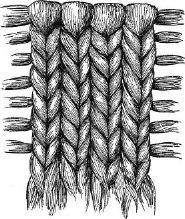
\includegraphics[scale=0.6]{./images/fig172.jpg}
\caption{Textiles from Arizona. }
\end{figure}

\section{Adding some more user helper macros}

It is expected that the user will produce a file, either through some automatic means or by typing it to hold the data. Deletion and insertion is simply via editing this file through a text editor. However, for completeness, we will write a few macros to help with maintenace of the database. These include macros for delete and modify record etc.

Another set of macros that one can use is to typet the records in lists and or tabulat forms, if required. Early books on archaelogy for example listed all the items in the following format, interspersed with comments and figures.
\smallskip


\hangindent3em
2520. (39510). A double globe jar or canteen. White ground, with ornamentations in black, as seen in Fig. 649. Depression in the center is probably designed to receive a band or cord to carry it with.
\smallskip

Although one is tempted to produce a list for these, the next item from such a book points otherwise:
\smallskip

\hangindent3em
2677-2678. 2677, (39617), and 2678, (39618). With flared and notched rim.
\smallskip

Before extending the database for such forms of descriptions, we can develop the typesetting part. I am sure that Lamport would have used a list, possibly due memory and space limitations and just re-use the \verb+\item+ command, in our case it is better to rather define a small macro
to cater for such items. The indentation can easily be achieved using \verb+\hangindent3em+ or a similar amount of measure.

\begin{verbatim}
\long\def\catno#1\par{
\par%
\hangindent3em\noindent
#1
}
\end{verbatim}


\def\catno#1#2{%
    \@hangfrom{#1. }#2
}


\DescribeMacro{\@hangfrom}\marg{text}   
\LaTeX\ provides a macro named \verb+\@hangfrom{<text>}+, that puts \marg{text} in a box, and makes a hanging indentation of the following material up to the first \verb+\par+. This Should be used in vertical mode.\footnote{See source2e, \texttt{ltsect.dtx}, pg 287.}

\begin{verbatim}
121 \def\@hangfrom#1{\setbox\@tempboxa\hbox{{#1}}%
122 \hangindent \wd\@tempboxa\noindent\box\@tempboxa}
\end{verbatim}

\medskip

\catno{289}{(39914). Fig. 397. Red ware, with white lines on the lower globe and decorations in black on the upper, with orifice in each globe.}

\catno{1289}{(39914). Fig. 397. Red ware, with white lines on the lower globe and decorations in black on the upper, with orifice in each globe.}


\makeatother

\section{Epiloque}

We have managed to write a database, sort it, typeset its contents in a structured or freeform manner
and on the way we have documented the code using a form of \textit{literate programing.} On top which
other language expects you to code your own ifs and for? 
The amount of code we wrote was very minimal and competes well with modern computer languages. 

Hope you had fun. Go and make beautiful books. 

\begin{figure}[htp]
\centering
{\color{thegray}
\fbox{\includegraphics[width=1\linewidth]{./images//pottery-figures.pdf}}}
\caption{Many books in the humanities have figure pages, with many different styles and numbering schemes. This page extract is from \textit{The Cypro-Phoenician pottery of the Iron Age. }  \citep{schreiber1971}}
\end{figure}


\begin{figure}[htp]
\centering
{\color{thegray}
\fbox{\includegraphics[width=1\linewidth]{./images/sample-tof.pdf}}}
\caption{Many books in the humanities have figure pages, with many different styles and numbering schemes. This page extract is from \textit{The Cypro-Phoenician pottery of the Iron Age. }  \citep{schreiber1971} and shows a specific way of numbering subfigures, including references.}
\end{figure}
\clearpage



 \subsection{Acknowledgements}

 Octavo is a modification of \texttt{classes.dtx} written by Leslie Lamport (1992),
 Frank Mittelbach (1994-97) and Johannes Braams (1994-97). As can be seen
 from the code, my own input is restricted to a tweaking of some parameters
 and true credit is due to Lamport, Mittelbach and Braams for their
 monumental efforts.



\begin{comment}
 \begin{thebibliography}{16}

 \bibitem{knuth98} Knuth,~D. 1998. \emph{Digital Typography}. CSLI 
 Publications, Stanford.

 \bibitem{rosarivo61} Rosarivo,~R. 1961. \emph{Divina proportio typographica}. 
 Scherpe, Krefeld.

 \bibitem{taylor98} Taylor,~P. 1998. \emph{Book design for \TeX\ users, Part 1: 
 Theory.} TUGBoat, 19:65--74.

 \bibitem{taylor99} Taylor,~P. 1999. \emph{Book design for \TeX\ users, Part 2:
 Practice.} TUGBoat, 20:378--389.

 \bibitem{town} Town,~L. \emph{Bookbinding by hand.} Faber \& Faber, London.

 \bibitem{tschichold87} Tschichold,~ J. 1987. \emph{Ausgew\"{a}hlte Aufs\"{a}tze
 \"{u}ber Fragen der Gestalt des Buches und der Typographie}. Birkh\"{a}user
 Verlag, Basel.

 \bibitem{williamson66} Williamson,~H. 1966. \emph{Methods of book design.} Oxford 
 University Press, Oxford.

 \bibitem{wilson01} Wilson,~P. 2001. \emph{The Memoir class for configurable
 typesetting.} CTAN. \url{macros\\latex\\contrib\\memoir} 

 \end{thebibliography}
\end{comment}





\chapter[Overflowing Figures into Margins]{OVERFLOWING FIGURES INTO MARGINS}

Most users of \TeX\ are accustomed to let the system position images, either on top or bottom of the page and occasionally use the [h] positioning directive to place the image at the exact location it appears in the text. Traditional typography placed the image in many different positions. It also occasionally overflowed the image into the margins. The image below, copied from the \textit{American Antiquarian}, was placed in the original publication as such. Tufte advocates the use of such techniques in displaying not only information, but also other material such as tables. The Tufte class is discussed extensively in other sections. It has almost a religious following attached to it and I have personally used it for business reports.\citep{seraphini}

\begin{figure}[htbp]
\leftskip-.07\textwidth\includegraphics[width=1.14\textwidth]{./images/elephant-long.jpg}\par

\begin{multicols}{4}
\myanmar

လူတိုင်းသည် တူညီ လွတ်လပ်သော ဂုဏ်သိက္ခါဖြင့် လည်းကောင်း၊ တူညီလွတ်လပ်သော အခွင့်အရေးများဖြင့် လည်းကောင်း၊ မွေးဖွားလာသူများ ဖြစ်သည်။ ထိုသူတို့၌ ပိုင်းခြား ဝေဖန်တတ်သော ဉာဏ်နှင့် ကျင့်ဝတ် သိတတ်သော စိတ်တို့ရှိကြ၍ ထိုသူတို့သည် အချင်းချင်း မေတ္တာထား၍ ဆက်ဆံကျင့်သုံးသင့်၏။
\end{multicols}
\centerline{\protect\textsc{Codex Seraphinianus, Mystery Procession \protect\citep{seraphini}}.}
\end{figure}

Almost as a matter of rule, the caption for these images was in small caps. Using small caps brought the caption into the easy attention of the reader, but it did not distract from the other elements of the page.
The image is not necessarily positioned symmetrically in the page, you can offset it to suit your taste, but in general, unless the image has any particular features that would make it look better offset rather than centered, is best positioned symmetrically. This can be automated, by writing a macro that measures the dimensions of the image and introduces a \verb+\leftskip+ so that the image can be shifted accordingly. A macro to achieve this is now described.


The image can be included by simply using a \verb+\skip-1.2cm+ or \verb+\leftskip-1.2cm+ :

\begin{verbatim}
\begin{figure}[htbp]
\leftskip-1.2cm\includegraphics{image}\par
\centerline{\textsc{Copper Sheath}}
\end{figure}
\end{verbatim}

\long\def\imghangleft#1#2{%
     \figure
     \leftskip-#2\textwidth\includegraphics[width=#1\textwidth]{./images/elephant-long.jpg}\par
     \centerline{\textsc{Codex Serafinianus}}
    \endfigure
}

\imghangleft{1.14}{.07}





